%%%%%%%%%%%%%%%%%%%%%%%%
%                                                                       %
% Verification and Validation   %
%                                                                        %
%%%%%%%%%%%%%%%%%%%%%%%%%

\chapter{Verification and Evaluation}
\label{chapter:validation}
%COMMENTED OUT AFTER TONY's REVIEW
%TONY: In this section, all you are doing is testing if your program generates a similar results as given by another program. There is no need to talk about the geological model or problem. Talking about diagenesis and any implication to petroleum system is out of question.

%During the development of this work, we have always been in contact with geochemists to present them the partial results of our geochemical speciation modelling software. We collected feedbacks regarding how to achieve a better software, as well as checking if our solution is fulfilling its purpose with consistent results. \\
%As final evaluation of this work, we selected an application relevant to petroleum systems. Many physical-chemical reactions happens during the generation, migration and storage of oil. \emph{Diagenesis} is the definition of the several processes that are involved and it is driven by multiple factors as temperature, pressure, mineral composition, water composition, activity of the solutes, pH, etc. 
%The \emph{diagenesis} is responsible for compaction and precipitation of minerals \cite{Tucker:01} and therefore, porosity, solubility and permeability of these reservoirs. The study of diagenesis is important because it allows to understand the geologic history of rocks, specially sedimentary rocks. In sedimentary rocks, the deposition of sediments are compacted in different layers and cemented by minerals that precipitate from reactions in a chemically very active environment. The \emph{diagenesis} reactions happens because the components are always trying to reach equilibrium, and therefore, they tend to interact with each others \cite{Burley:85}.
%Using geochemical modelling softwares is a powerful tool to understand the diagenetic processes and the natural conditions that occur in this natural environment. The goal is to numerically model this environment and analyse the results of the diagenetic reactions with a petrographic analysis of the modeled reservoirs.


%Análise geologica da aplicação do SHPECK feita pela Mara
In order to test and evaluate the simulator, we model the diagenetic reactions observed in Snorre Field reservoir sandstones of Norwegian North Sea. The main reservoir horizons of the field are the fluvial sandstones in the upper member of the Upper Triassic Lunde Formation and the Upper Triassic to Lower Jurassic Statfjord Formation \cite{Hollander:87}. The sandstones sampled for this study, according to Morad \cite{Morad:90}, belong to the upper member of the Lunde Formation. The sandstones are dominantly fine- to medium-grained and arkosic with framework constituents of quartz (40-80\%), K-feldspar (5-12\%), plagioclase (15-45\%), muscovite, biotite and clay minerals that include smectite, mixed-layer clay minerals, chlorite and subordinate amounts of kaolinite and illite. Subordinate rock fragments include intraformational mudstone and carbonate clasts and extrabasinal grains of quartz-feldspar-mica aggregates that probably represent granitic rocks and/or schist or gneisses. Mica and detrittal clay minerals seldom make up more than 2\% of the total mineral content in the sandstones. Diagenetic clay minerals include pore-filling kaolinite and pore-lining smectite, mixed-layer chlofite-smectite, and chlorite. Other cements include the carbonates (0.0-25\%) which play a significant role in porosity reduction in some of the sandstones. Authigenic overgrowths are primarily quartz, anatase and minor albite, pyrite and barite.

\section{Case Study}
For the model’s validation, the diagenetic reactions observed in Snorre Field reservoir sandstones, Norwegian North Sea was simulated. The modeling set up and results given in Morad \cite{Morad:90} describes the texture, origin, chemistry of the sandstones reservoirs in terms of the water composition and temperature. Against this \emph{SHPECK}'s results were examined.

The descriptions presented in \cite{Morad:90} of the diagenetic reactions that take place in the Snorre Field allows us to generate a computationally comparative study. We model and compare the same diagenetic environment using \emph{SHPECK}, \emph{PHREEQC} and \emph{MINTEQA2}. The water composition is detailed in \cite{Nordstrom:79}.

We approach the environment described above following two methodologies: experimental and computational. The first one analyzes and compare the behavior of \emph{SHPECK} with petrographic analysis through thin sections (available in \cite{Morad:90}). The second treats the direct comparison of \emph{SHPECK}'s result side-by-side with other software's.

\subsection{Experimental validation of Shpeck}
As stated in \cite{Morad:90}, the model presented in \cite{Egeberg:88} calculates activities of the various ions of formations waters using ion association model (originally described in \cite{Wigley:77}). 
The thermodynamics data used are given in \cite{Helgeson:74a},  \cite{Helgeson:74b}, \cite{Helgeson:76}, \cite{Waltter:77}, \cite{Helgeson:78} and \cite{Helgeson:81}.

The activity diagram generated for a known temperature and log activity ratio of Potassium to Sodium ions of \cite{Aagaard:90}  is provided as input to \emph{SHPECK} model (Figure ~\ref{fig:tempXactratio}). The results show a consistent pattern: as the temperature rises the potassium activity gets higher over sodium’s, which means that the phases associated to the ion potassium (i.e. K-feldspar, Illite, etc) are dissolving.


\begin{figure}[ht!]
\centering
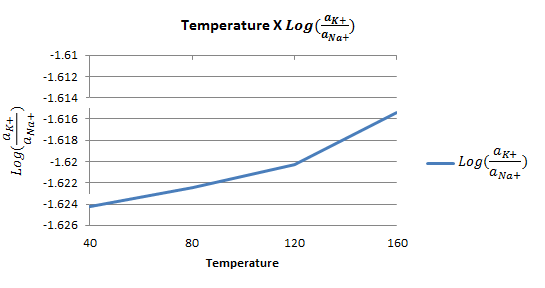
\includegraphics[width=100mm]{figures/tempXactratio.png}
\caption{Log activity ratio of Potassium to Sodium ions using the results from \emph{SHPECK}}
\label{fig:tempXactratio}
\end{figure}

% QUESTION:
% LEO: I wasn't sure if I should put the figure from aagaard's in order to really prove that our results are consistent.... I don't like the idea of putting someone else's graph in here..
%TONY: You cannot use a published figure without getting the copyright waive from the publisher. What you can do is to replicate the figure of Aagaard using your own resources.


\subsection{Computational comparative study} 
By modeling the same environment using three distinct software packages, we attain a relevant comparison among the numerical methods and algorithms.
Chemical composition of the water adopted in the models is taken from  \cite{Nordstrom:79} which provides the chemical composition of the seawater (table ~\ref{tab:nordstrom}). The comparative study tested temperatures that have varied from $100^o$C to $100^o$C. In \emph{MINTEQA2}, due to limitations of its thermodynamics equilibrium database, the maximum temperature available is $100^o$C.

\begin{table}
\caption{Chemical composition of the solution in the sea water at $25^o$ in $mM/L$C }
\label{tab:nordstrom}
\centering
\begin{tabular}{r|c|c|c|c|c|c|c|c|c}
\ce{Al^{3+}} & \ce{K^+} & \ce{Na^+} & \ce{Ca^{2+}} & \ce{Mg^{2+}} & \ce{Fe^{2+}} & \ce{SiO_2}&  
\ce{SO_4^{2-}} & \ce{Cl^-} & pH
    \\ \hline
7.59e-5 & 10.45 & 479.32 & 10.53 & 54.39 & 3.66e-5 & 0.073 & 28.893 & 559.5 & 8.22
\end{tabular}
\end{table}

We aim to model the diagenetic processes that best represent the behavior of ions in the water-rock interactions. Figures ~\ref{fig:na+},~\ref{fig:cl-},~\ref{fig:mg+2} and ~\ref{fig:ca+2} present the most representative ions of the solution. It is possible to see that the behavior of \emph{SHPECK} is similar to  both \emph{PHREEQC} and \emph{MINTEQA2} in most of the cases, especially in temperatures under $100^o$C. We observe a more dissimilar behavior between \emph{SHPECK} and \emph{PHREEQC} in temperatures higher than $100^o$C, but the results were never completely opposite. This can be explained by the temperature intervals  where the equilibrium constant \emph{K} is not completely defined.  

This is a known issue from \emph{LLNL} thermodynamic dataset: sometimes equilibrium constants have no measures in literature and are treated as unknown. \emph{SHPECK} adopts the nearest equilibrium constant known value. Unfortunately we do not have access to the whole software’s details in order to describe how they treat this issue.

\begin{figure}[ht!]
\centering
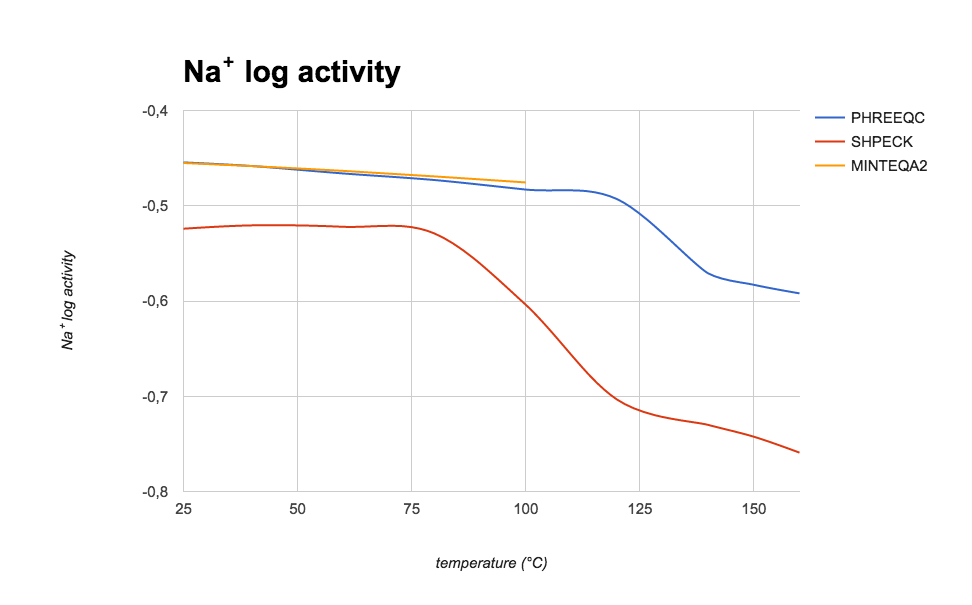
\includegraphics[width=140mm]{figures/na+.png}
\caption{\ce{Na^+} log activity comparative study}
\label{fig:na+}
\end{figure}

\begin{figure}[ht!]
\centering
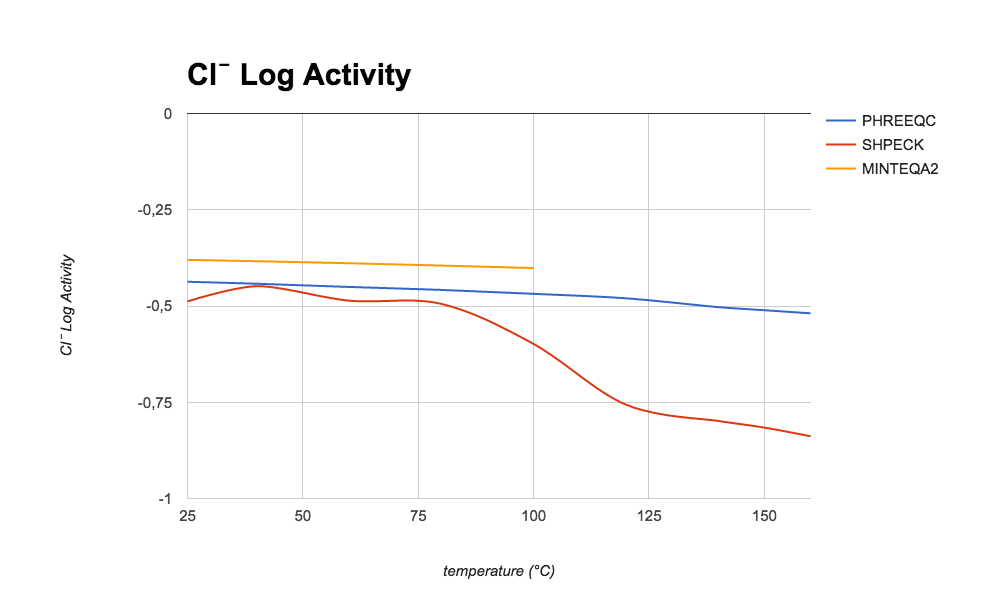
\includegraphics[width=140mm]{figures/cl-.png}
\caption{\ce{Cl^-} log activity comparative study}
\label{fig:cl-}
\end{figure}

\begin{figure}[ht!]
\centering
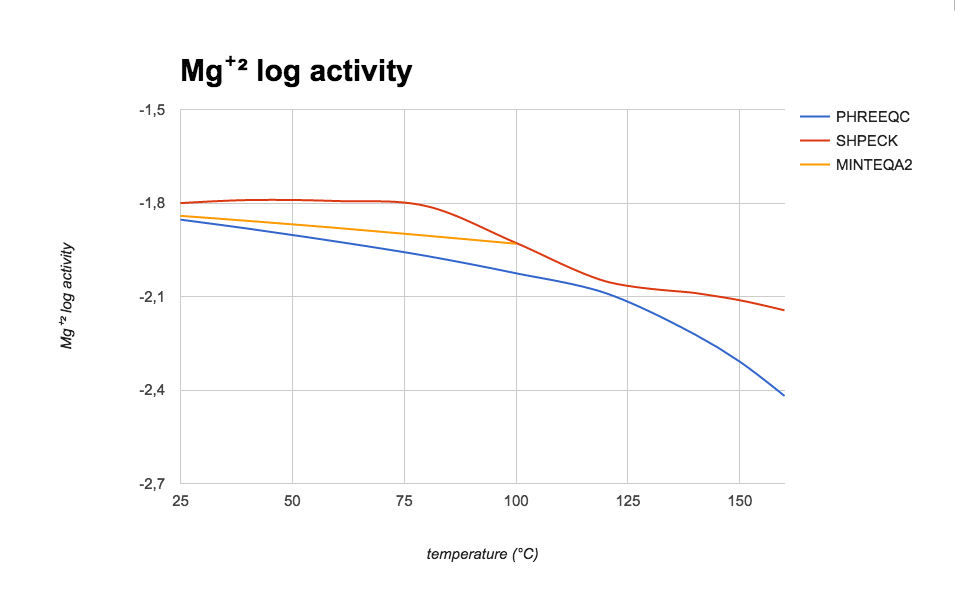
\includegraphics[width=140mm]{figures/mg+2.png}
\caption{\ce{Mg^{+2}} log activity comparative study}
\label{fig:mg+2}
\end{figure}

\begin{figure}[ht!]
\centering
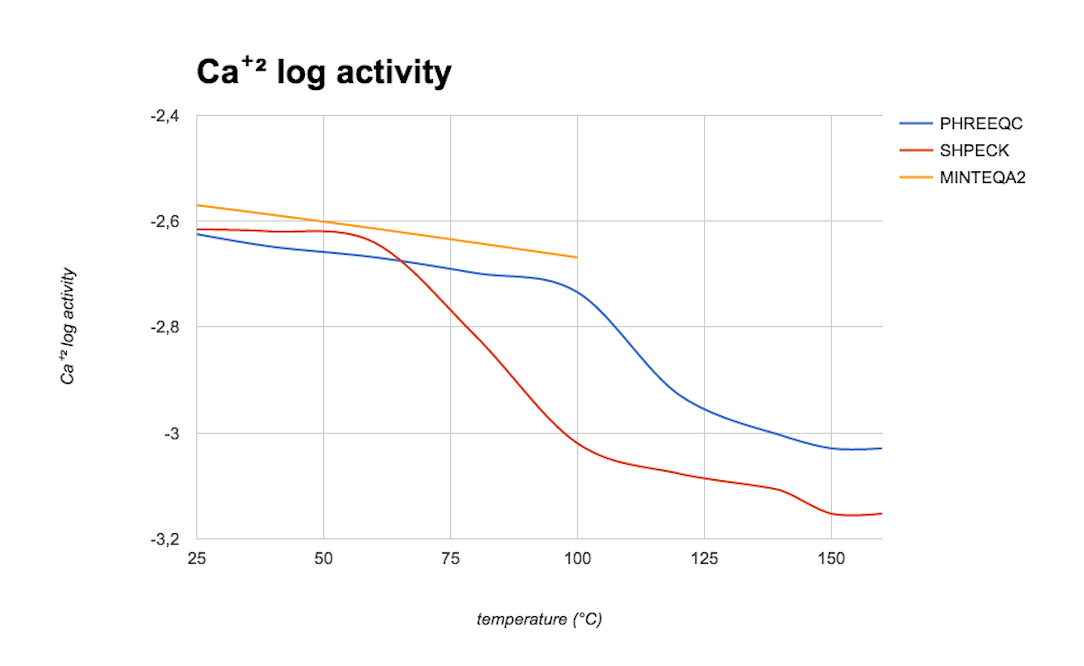
\includegraphics[width=140mm]{figures/ca+2.png}
\caption{\ce{Ca^{+2}} log activity comparative study}
\label{fig:ca+2}
\end{figure}

\begin{figure}[ht!]
\centering
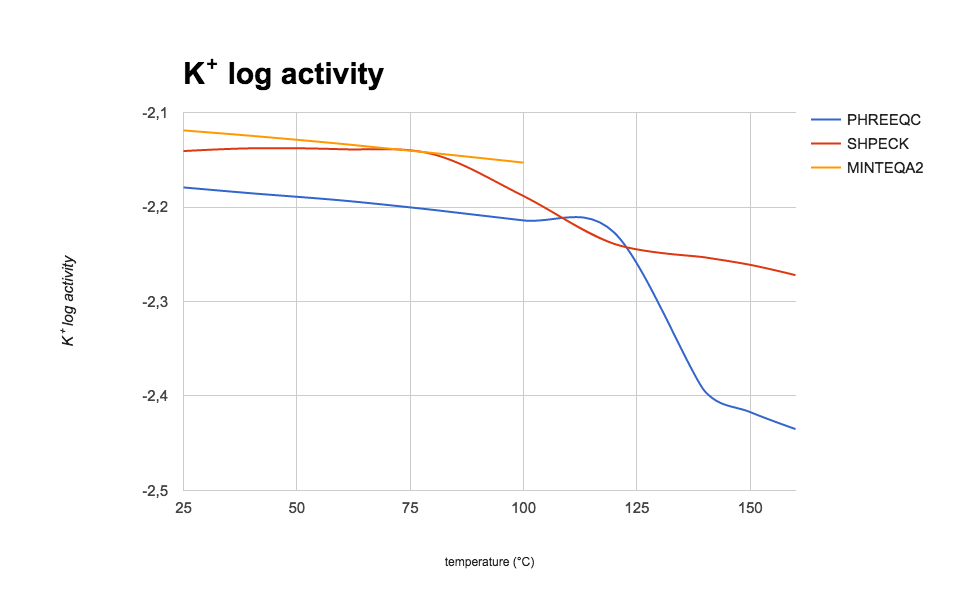
\includegraphics[width=140mm]{figures/k+.png}
\caption{\ce{K^+} log activity comparative study}
\label{fig:k+}
\end{figure}

\begin{figure}[ht!]
\centering
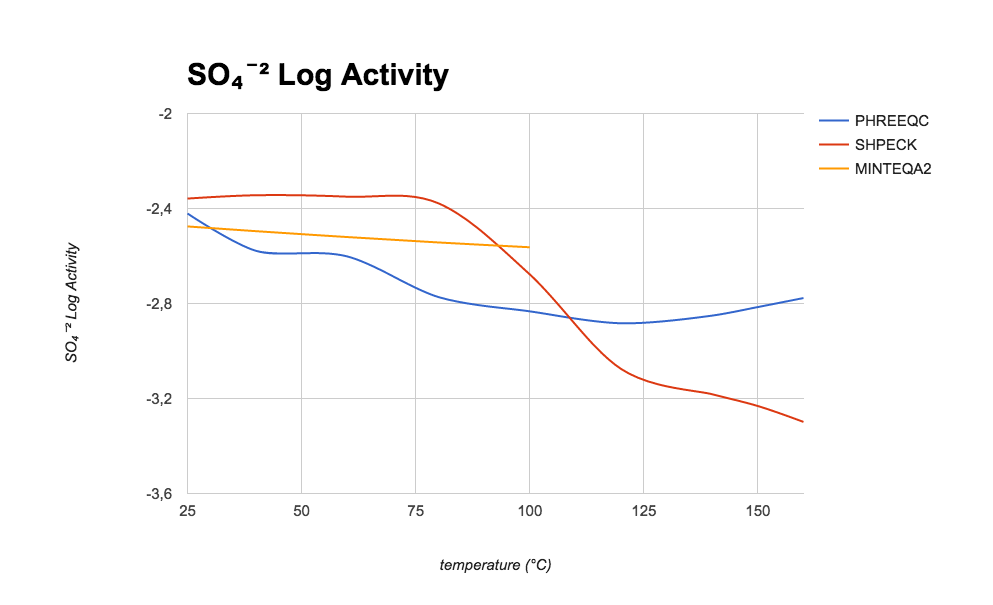
\includegraphics[width=140mm]{figures/so4-2.png}
\caption{\ce{SO_4^{-2}} log activity comparative study}
\label{fig:so4-2}
\end{figure}


\section{Database Evaluation}
The geochemical models used for comparison studies use text files as the database. The goal of this section is to make clear the difference and - more importantly - the benefits of \emph{SHPECK}'s relational database. Most of the information inside a geochemical database is related to each other (i.e. a mineral phase is described by a reaction, a reaction is composed by solute species, and a solute species is composed of chemical elements). \emph{SQLite} databases are naturally a structure where the data can be related to each other, and this significantly improvements the performance and robustness of the application. On \emph{SQLite} databases, the data can be accessed using \emph{SQL} queries that reduce the complexity and increase the speed on information retrieval - code~\ref{cod:sqlQuery} shows a complex \emph{SHPECK}'s \emph{SQLite} query. Text database files only allow sequential access to the information that it contains. In relation databases, the \emph{SQL} language allows random access and it  is used to selectively locate needed data.


\begin{minipage}{0.8\linewidth}
\begin{lstlisting}[frame=single, label=cod:sqlQuery, caption=\emph{SHPECK}'s \emph{SQLite} example query]
SELECT compoundsComposition.element, compoundsComposition.name, compoundsComposition.stoich, compounds.eqConstant, termoPolynom.zero, termoPolynom.one, termoPolynom.two, termoPolynom.three, termoPolynom.four, termoPolynom.five, termoPolynom.six, termoPolynom.seven FROM termoPolynom, compoundsComposition, compounds WHERE compoundsComposition.name = compounds.name AND termoPolynom.name = compounds.name AND compounds.name = XXXXX;
\end{lstlisting}
\end{minipage}

Important to note that at each simulation the value ”XXXX” in code 1 is updated to the simulation’s solute name. Also interesting to point that the information fetched with this query comes from three different tables and, in only one query, many relevant information for the simulation is fetched.

\subsection{Configuration setup}
Our experiments' methodology was first defining what was the information necessary from the database to generate the set of reactions. After that, we define the order that this information was necessary and how to fetch it. At the end, the measurement metric is to verify how long the program was idle waiting for this information and when it finally was available. In both the relational database and flat file experiments, we used the \emph{NNLN} thermodynamic dataset.
The tests were executed on a MacBook air, i7 processor, 1.7GHz, 8GB RAM running OS X 10.9.3.

\subsection{Time analysis of fetching information}
The objective of the time analysis is to measure how long it takes to fecth the same information from different types of database. The response time is considered as the sum of the processing time and the time waiting for the availability of the resource. It is necessary to understand that until the software has received the information requested from the database it is inactive and in a standby mode. In order to analyze the response time within a geochemical analysis point of view, we discuss not only the access time but also the implications of that information. 

When fetching any information from a thermodynamic dataset, it is important to take into consideration additional allied data will also have to be retrieved. For example, when fetching a reaction (as expressed in equation~\ref{reaction}) data, the basic information consists of the compounds that take part on this reaction and the related stoichiometric values. Behind this action, the database must also provide information about the compounds itself (i.e. charge, ion size, mole weight, elements in that specie, formula, mole volume) as well as the reaction (i.e., thermodynamic equilibrium constant coefficients, etc).

Figure ~\ref{fig:timeXaccess} indicates the time elapsed (in seconds) that it takes to retrieve the necessary information related to a chemical reaction from the database. In this example, we simulated from 20 to 580 randomly selected reactions in the database. It is possible to see that \emph{SHPECK}'s database has improved approximately 40\% in the average time elapsed to fetch the information if compared to the regular text file database used by other simulation packages.

\begin{figure}[ht!]
\centering
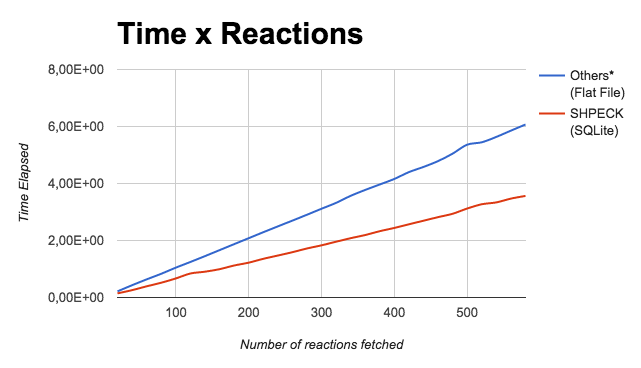
\includegraphics[width=140mm]{figures/timeXreactionAccess.png}
\caption{Time elapsed in seconds X Reactions Accessed}
\label{fig:timeXaccess}
\end{figure}

\newpage

\section{Summary}
\begin{itemize}
    \item Diagenesis: This term refers to chemical and physical changes taking place in a rock due to chemical reactions. In this study we reproduce the diagenetic reactions observed in Snorre Field reservoir sandstones, Norwegian North Sea. 
    The environment modeled is described in \cite{Morad:90} and the chemical composition of the water in \cite{Nordstrom:79}.
    \item Comparative study: We performed a comparative study of \emph{SHPECK} and other available geochemical speciation software. The results prove that \emph{SHPECK} produce comparable results. The discrepancies are minimal and the differences can be justified by the software-specific implementations of the mathematical and computational treatment to the set of equations and other parameters. 
    \item Database evaluation: The lack of a relational database in the geochemical modeling software makes it clear that none of the existing options were developed with emphasis on a computer science emphasis. \emph{SHPECK} uses a \emph{SQLite} database specially developed to support a geochemical speciation modeling software. This software design option enables the software to achieve efficient performance, and handle complex data queries and retrieval. A comparative graph highlights the advantages in time elapsed by the number of reactions requested.
\end{itemize}